% !TeX spellcheck = cs_CZ
\section{Jednočinný blokující měnič}\label{ENZ:ssec_01}\hypertarget{ENZ:ssec_01}
  Základem tohoto měniče je „invertující měnič se společnou tlumivkou“ z kapitoly \ref{aes:sec003}. 
  Všimneme si, že z původního schématu (obr. \ref{enz:fig_007a}) vymizela tlumivka, jejíž funkci 
  nyní zastane transformátor. 
  \begin{figure}[ht!]
    \centering
    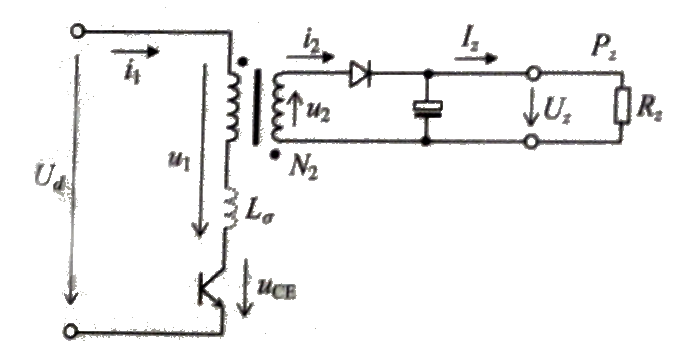
\includegraphics[width=0.6\linewidth]{flyback_sch.png}
    \caption{Základní zapojení jednočinného blokujícího měniče.}
    \label{enz:fig_008}
  \end{figure} 
  Princip činnosti je vlastně úplně stejný, pokud si uvědomíme, že jádro nynějšího transformátoru 
  je magnetováno stejně jako jádro tlumivky na obr. \ref{enz:fig_007a}, viz. průběh $i_L(t)$ v 
  obr. \ref{enz:fig_007b} a průběh $\Phi_\mu(t)$ v obr.\ref{enz:fig_008}. Jediný rozdíl je v tom, 
  že stejných magnetických poměrů je nyní dosaženo pomocí dvou vinutí místo původního jednoho (v 
  době $t_1$ pomocí $L_1$ a v době $t_2$ pomocí $L_2$). Tím se dosáhne galvanického oddělení. 
  Vznikl tak transformátor, ovšem režim jeho činnosti je takový, že magnetické účinky v jádře se 
  podobají tlumivce. Režim je zcela odlišný od režimu transformátoru v propustných měničích.
 
  \begin{figure}[ht!]
    \centering
    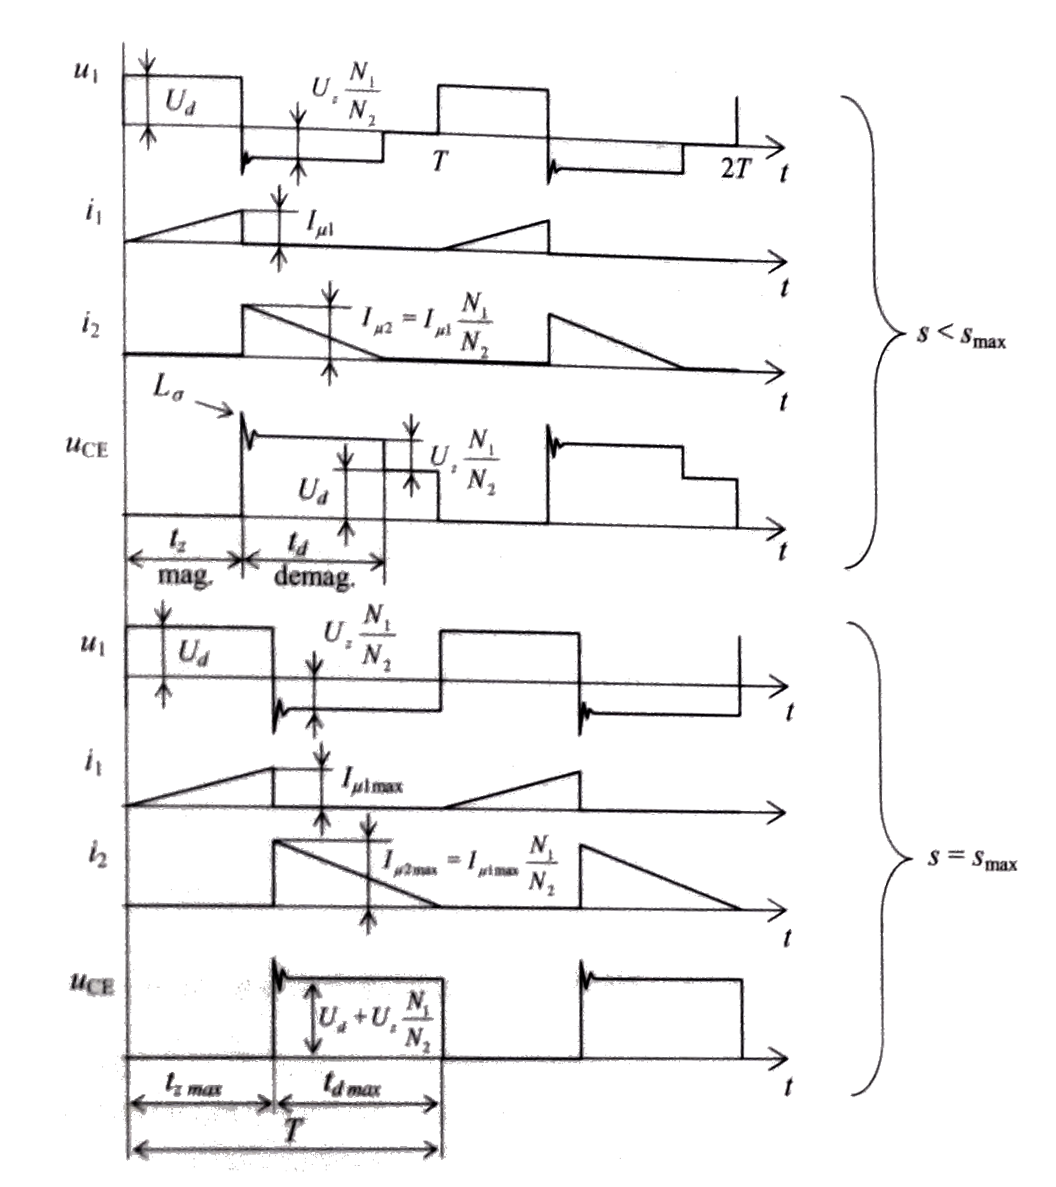
\includegraphics[width=\linewidth]{flyback_wave.png}
    \caption{Časové průběhy všech důležitých veličin v blokujícím měniči.}
    \label{enz:fig_009}
  \end{figure} 
  Indukčnost \(L_\sigma\) představuje \emph{parazitní rozptylovou indukčnost transformátoru}. 
  Rozptylová indukčnost je nežádoucí, protože způsobuje přídavný napěťový překmit na tranzistoru 
  v okamžiku vypínání. Velikost překmitu roste s velikostí proudu, tedy s velikostí přenášeného 
  výkonu. To je značná nevýhoda blokujících měničů.
  
  Činnost měniče vyplývá z časových průběhů na obr. \ref{enz:fig_009}. V horní části jsou 
  nakresleny průběhy při menší střídě \(\delta\), v dolní jsou tytéž průběhy, ale při maximální 
  střídě. V časovém intervalu \(t_z\) je tranzistor sepnut, tudíž probíhá \emph{magnetizace} 
  transformátoru proudem \(i_1\) pomocí \emph{primárního} vinuti. Dioda sekundárního usměrňovače 
  je v té době zavřena, zátěž je odpojena od transformátoru a napájena pouze z nabitého 
  kondenzátoru. V intervalu \(t_d\) je tranzistor vypnut, tudíž probíhá \emph{demagnetizace} 
  transformátoru pomocí \emph{sekundárního} vinutí. Dioda je v té době otevřena a kondenzátor je 
  napájen demagnetizačním trojúhelníkovým proudovým pulsem \(i_2\). V té chvílí je sekundární 
  vinutí přes diodu připojeno na \emph{konstantní} napětí \(U_z\) kondenzátoru a tímto napětím je 
  demagnetováno. Aby bylo napětí konstantní, kondenzátor musí mít dostatečně velkou kapacitu. 
  Magnetizační proud \(i_1\), roste \emph{lineárně} s časem, protože je integrálem z 
  \emph{konstantního} napětí \(+U_d\). Podobně demagnetizační proud \(i_2\) klesá \emph{lineárně} 
  s časem, protože je integrálem z \emph{konstantního} napětí \(-U_z\). V dolní části obr. 
  \ref{enz:fig_009} jsou nakresleny průběhy při maximální střídě \(\delta_{max}\). Je to mezní 
  stav, při kterém je demagnetizace dokončena přesně na konci pracovní periody \(T\) a 
  magnetizační tok právě zaniká. Teoreticky je možné střídu zvětšit, pak nedojde k úplné 
  demagnetizaci a transformátor začne pracovat v režimu \emph{nepřerušovaného} spojitého 
  magnetického toku, viz horní průběh na obr. \ref{enz:fig_010}. V tom případě bude sice 
  přenášený výkon větší, ovšem za cenu, že režim je \emph{neoptimální}. Důvod spočívá v tom, že 
  minimální tok \(\Psi_{min}\) sice vzroste, ale maximální zdvih pilovitého zvlnění 
  \(\Delta\Psi\) se zvětšit nemůže a zůstává \emph{konstantní}. Energie \(\Delta W\), přenesená v 
  jednom pracovním cyklu, je dána rovnicí
  \begin{align}
    \Delta W 
      &= \frac{1}{2}\frac{\Psi_{max}^2}{L_1} 
       - \frac{1}{2}\frac{\Psi_{min}^2}{L_1}   
       = \frac{1}{2}\frac{(\Psi_{min}+\Delta\Psi)^2}{L_1} 
       - \frac{1}{2}\frac{\Psi_{min}^2}{L_1}   \nonumber \\
      &= \frac{1}{2L_1}\left(2\Psi_{min}\Delta\Psi+\Delta\Psi^2\right) \label{ENZ:eq_001}
  \end{align}
  
  \begin{figure}[ht!]
    \centering
    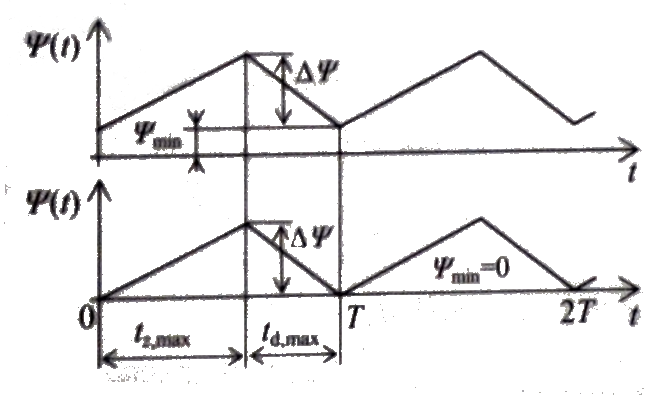
\includegraphics[width=0.6\linewidth]{flyback_tok.png}
    \caption{Spřažený tok transformátoru při podmínce \(\Psi_{min}>0\) a \(\Psi_{min}=0\)}
    \label{enz:fig_010}
  \end{figure} 
  
  Vidíme, že množství přenášené energie \(\Delta W\) je dáno \emph{druhou} mocninou zdvihu 
  \(\Delta\Psi\), ale pouze \emph{první} mocninou minimální hodnoty \(\Psi_{min}\). Růst hodnoty 
  \(\Psi_{min}\) je proto energeticky málo účinný a tudíž nevýhodný. Optimální stav nastává při 
  podmínce \(\Psi_{min} = 0\). Měnič bude analyzován a navrhován právě při dodržení této podmínky.
  \begin{align}
    \shortintertext{Pracovní střídaje definována rovnici}
    \delta       &= \frac{t_z}{T}. \label{ENZ:eq_002} \\
    \shortintertext{Pro maximální střídu zřejmé platí vztah}
    \delta_{max} &= \frac{t_{z_{max}}}{t_{z_{max}}+t_{d_{max}}}
                  = \dfrac{1}{1+\dfrac{t_{d_{max}}}{t_{z_{max}}}}. \label{ENZ:eq_003} \\
    \shortintertext{V době zapnutí poroste magnetizaění proud \(i_1\) se strmostí}
    \der{i_1}{t} &= \frac{I_{{\mu1}_{max}}}{t_{z_{max}}} 
                  = \frac{U_d}{L_1}  \label{ENZ:eq_004} \\
    \shortintertext{V době vypnutí bude magnetizaění proud \(i_2\) klesat (v absolutní hodnotě) 
                    se strmostí}
    \der{i_2}{t} &= \frac{I_{{\mu2}_{max}}}{t_{d_{max}}} 
                  = \frac{U_z}{L_2}  \label{ENZ:eq_005}
  \end{align}    
  Z rovnic (\ref{ENZ:eq_005}) a (\ref{ENZ:eq_004}) plyne pomocná rovnice
  \begin{align}
    \frac{t_{d_{max}}}{t_{z_{max}}} 
      &= \frac{U_d L_2 I_{{\mu2}_{max}}}{U_z L_1 I_{{\mu1}_{max}}} \label{ENZ:eq_006} \\
    \shortintertext{Má-li transformátor těsnou vazbu \(k \rightarrow 1\), zřejmě platí}  
    \frac{L_2}{L_1} = \frac{N_2^2}{N_1^2} \label{ENZ:eq_007} \\
    \shortintertext{Z proudového převodu transformátoru plyne}
    \frac{I_{{\mu2}_{max}}}{I_{{\mu1}_{max}}}
      &= \frac{N_1}{N_2}. \label{ENZ:eq_008} \\
    \shortintertext{Po dosazení rovnic (\ref{ENZ:eq_008}) a (\ref{ENZ:eq_007}) do
                   (\ref{ENZ:eq_006}) získáme vztah}
    \frac{t_{d_{max}}}{t_{z_{max}}} 
      &= \frac{U_d N_2}{U_z N_1}  \label{ENZ:eq_009} \\
    \shortintertext{Rovnici (\ref{ENZ:eq_009}) dosadíme do (\ref{ENZ:eq_003}). Tak získáme výraz 
                    pro maximální střídu:}
    \delta_{max} 
      &= \dfrac{1}{1+\dfrac{U_d N_2}{U_z N_1}}. \label{ENZ:eq_010} 
  \end{align}
  V době demagnetizace se sekundární demagnetizační napětí \(U_z\) přetransformuje s převodem na 
  primár a zde se přičte k mezilehlému napětí \(U_d\). Tranzistor je namáhán součtem těchto 
  napětí:
  \begin{align}
    U_{CE_{max}} &= U_d + U_z\frac{N_1}{N_2}   \qquad \Rightarrow \qquad 
    U_z\frac{N_1}{N_2} = U_{CE_{max}} - U_d    \label{ENZ:eq_011} \\
    \shortintertext{Rovnici (\ref{ENZ:eq_011}) dosadíme do (\ref{ENZ:eq_010}). Pak bude mít 
                    maximální střída velikost}
    \delta_{max} &= 1-\frac{U_d}{U_{CE_{max}}} \label{ENZ:eq_030}
  \end{align}
  Napětí \(U_d\) je zadáno. Maximální pracovní napětí tranzistoru \(U_{CE_{max}}\) je nutno 
  zvolit s ohledem na bezpečný provoz. Z rovnice (\ref{ENZ:eq_011}) plyne, že musí být bohužel 
  vždy splněna nerovnost
  \begin{equation}\label{ENZ:eq_012}
   U_{CE_{max}} > U_d,
  \end{equation}
  jinak nemůže měnič vůbec pracovat. Na hladině \(U_d = \SI{350}{V}\) se volí nejvýše 
  \(U_{CE_{max}} =  2\cdot U_d\) potom vychází \(\delta_{max} = 0,5\). Na hladině \(U_d = 
  \SI{600}{V}\) se musí volit poměr daleko menší, např. \(U_{CE_{max}} =  1,1\cdot U_d\) protože 
  běžně lze použít tranzistory MOSFET se závěrným napětím okolo \(\SI{800}{V}\). Ale i tak, 
  vychází maximální střída pouze \(\delta_{max} = 0,09\), což vede k naprosto neoptimálnímu 
  návrhu měniče. Potřebný počet sekundárních závitů plyne z rovnice (\ref{ENZ:eq_011}), případně 
  z rovnice (\ref{ENZ:eq_010}):
  \begin{equation}\label{ENZ:eq_013}
    N_2 = N_1\frac{U_z}{U_{CE_{max}}-U_d}, \qquad 
    N_1 = N_2\frac{U_z}{U_d}\frac{1-\delta_{max}}{\delta_{max}}
  \end{equation}
  
  \subsection{Návrh transformátoru}
    Výkon přenášený transformátorem je nutno určit pomocí magnetizační energie a pracovního 
    kmitočtu. Ze vztahu (\ref{ENZ:eq_002}) vyplývá pomocná rovnice
    \begin{align}
      t_z      &= \delta T = \frac{\delta}{f}.         \label{ENZ:eq_014} \\ 
      \shortintertext{Ze vztahu (\ref{ENZ:eq_004}) plyne další pomocná rovnice} 
      I_{\mu1} &= \frac{U_d t_z}{L_1}.                 \label{ENZ:eq_015} \\ 
      \shortintertext{Energie, načerpaná v době sepnutí primárním vinutím a bezeztrátově 
                      přenesená v jednom pracovním cyklu do zátěže, má zřejmě velikost}
      W_{L1}   &= \frac{1}{2}L_1I_{\mu1}^2 
                = \frac{1}{2}U_dI_{\mu1}t_z.           \label{ENZ:eq_016} \\
      \shortintertext{Má-li pracovní cyklus periodu \(T\), pak \emph{střední} neboli \emph{činný} 
                      výkon, přenášený do zátěže, bude}
      P_z      &= \frac{W}{T} = \frac{1}{2}U_dI_{\mu1}\frac{t_z}{T} 
                = \frac{1}{2}U_dI_{\mu1}\delta.        \label{ENZ:eq_017} \\
      \shortintertext{Do rovnice (\ref{ENZ:eq_017}) dosadíme (\ref{ENZ:eq_015}). Po úpravě 
                     získáme vztah}
      P_z      &= \frac{U_d^2\delta}{2L_1}t_z
                = \frac{U_d^2\delta}{2L_1}\frac{t_z}{fT}
                = \frac{U_d^2\delta}{2L_1}\frac{\delta}{f}
                = \frac{U_d^2\delta^2}{2fL_1}.          \label{ENZ:eq_018}
    \end{align}
    Potom bude transformátor schopen přenést zvolený maximální výkon\footnote{Blokující měnič 
    nemůže být nad tuto zvolenou hodnotu ani krátkodobě přetěžován - na rozdíl od propustných 
    měničů.} při maximální střídě:
    \begin{align}
      P_{z_{max}} &= \frac{U_d^2\delta_{max}^2}{2fL_1}           \label{ENZ:eq_019} \\ 
      \shortintertext{Tentýž maximální výkon lze též vyjádřit rovnicí (\ref{ENZ:eq_017}):}
      P_{z_{max}} &= \frac{1}{2}U_d I_{{\mu1}_{max}}\delta_{max} \label{ENZ:eq_020} \\
      \shortintertext{Z rovnice (\ref{ENZ:eq_019}) plyne požadovaná velikost primární indukčnosti}
      L_1         &= \frac{U_d^2\delta_{max}^2}{2fP_{z_{max}}}   \label{ENZ:eq_021} \\
      \shortintertext{Z rovnice (\ref{ENZ:eq_020}) plyne maximální velikost primárního 
                      magnetizačního proudu}
      I_{{\mu1}_{max}} &= \frac{2P_{z_{max}}}{U_d\delta_{max}}   \label{ENZ:eq_022} \\
      \shortintertext{Tentýž primární magnetizační proud (trojúhelníkového tvaru) má efektivní 
                      hodnotu}
      I_{{\mu1}_{ef}} &= I_{{\mu1}_{max}}\sqrt{\frac{\delta_{max}}{3}} \label{ENZ:eq_023}
    \end{align}
    Rovnice (\ref{ENZ:eq_021}), (\ref{ENZ:eq_022}) a (\ref{ENZ:eq_023}) jsou pro optimální návrh 
    transformátoru stěžejní. Návrh transformátoru je pak naprosto stejný jako návrh tlumivky 
    na feromagnetickém jádře se vzduchovou mezerou podle kapitoly 12. Tam byly vstupními 
    hodnotami pro návrh rovněž indukčnost \(L_1\) a proud \(I_{max}\), odpovídající indukci 
    \(B_{max}\). Jediný rozdíl je v tom, že v okně jádra transformátoru je nutno pamatovat i na 
    existenci sekundárního vinutí, které zřejmě zabere polovinu plochy okna. Proto je nutno 
    modifikovat původní rovnici (12.2.1-3) pro návrh tlumivky, kterou zde znovu uvedeme:
    \begin{align}
      S_0S_j &= \frac{LI_{max}^2k_z}{k_{p_{Fe}}k_{p_{Cu}}B_{max}\sigma} 
             =  \frac{LI_{max}I_{ef}}{k_{p_{Fe}}k_{p_{Cu}}B_{max}\sigma}. \label{ENZ:eq_024}  \\
      \shortintertext{do tvaru}
      \frac{S_0}{2}S_j 
             &= \frac{L_1I_{{\mu1}_{max}}I_{{\mu1}_{ef}}}{k_{p_{Fe}}k_{p_{Cu}}B_{max}\sigma}
              = \frac{L_1I_{{\mu1}_{max}}^2}{k_{p_{Fe}}k_{p_{Cu}}B_{max}\sigma}
                \sqrt{\frac{\delta_{max}}{3}}.                           \label{ENZ:eq_025}  \\
      \shortintertext{Činitel plnění feritového jádra je roven jedné. Rovnici poté upravíme do 
                      konečné podoby}
      S_0S_j &=2\sqrt{\frac{\delta_{max}}{3}} 
                \frac{L_1I_{{\mu1}_{max}}^2}{k_{p_{Cu}}B_{max}\sigma}
                \qquad [\si{m^4};\si{H},\si{A},\si{T},\si{A\per\m^2}].   \label{ENZ:eq_026}  \\
      \shortintertext{Dosadíme-li do této rovnice vztahy (\ref{ENZ:eq_021}) a (\ref{ENZ:eq_022}), 
                      získáme druhou podobu rovnice:}
      S_0S_j &=4\sqrt{\frac{\delta_{max}}{3}} 
                \frac{P_{z_{max}}}{k_{p_{Cu}}fB_{max}\sigma}
                \qquad [\si{m^4};\si{W},\si{Hz},\si{T},\si{A\per\m^2}].  \label{ENZ:eq_027}
    \end{align}
    Zdálo by se, že je výhodné volit co nejmenší maximální střídu \(\delta_{max}\). Avšak není to 
    vhodné, protože podle rovnice (\ref{ENZ:eq_022}) pak bude příliš veliký magnetizační proud 
    (proudové namáhání tranzistoru). Z rovnic (\ref{ENZ:eq_021}) a (\ref{ENZ:eq_022}) plyne, že 
    transformátor musí mít \textbf{vzduchovou mezeru}, pokud je navržen \emph{optimálně}. 
    Magnetická energie, načerpaná při zapnutí tranzistoru, se totiž nejsnáze ukládá do vzduchové 
    mezery, nikoli do feromagnetika. Proto lze z 12. kapitoly převzít a modifikovat rovnice 
    (12.1.1-3), (12.1.2-3) pro výpočet závitů a délky vzduchové mezery:
    \begin{align}
      N_1 &= \frac{L_1I_{{\mu1}_{max}}}{B_{max}S_j}          \nonumber          \\
      l_v &= \frac{N_1\mu_0I_{{\mu1}_{max}}}{B_{max}} 
           - \frac{l_{Fe}}{\mu_{r_{Fe}}},                    \label{ENZ:eq_028} \\
      \shortintertext{nebo}
      l_v &= \frac{L_1\mu_0I^2_{{\mu1}_{max}}}{B_{max}S_j} 
             - \frac{l_{Fe}}{\mu_{r_{Fe}}},                  \label{ENZ:eq_029}  
    \end{align}
    Postup při návrhu celého měniče je následující:
    \begin{enumerate}\addtolength{\itemsep}{-0.5\baselineskip}
      \item Je zadáno \(U_z\), \(P{z_{max}}\) ,\(U_z\)
      \item Volíme \(U_{CE_{max}}\),\(f\), \(B_{max}\).
      \item Podle rovnice (\ref{ENZ:eq_030}) určíme maximální střídu \(\delta_{max}\).
      \item Podle rovnic (\ref{ENZ:eq_021}) a (\ref{ENZ:eq_022}) určíme \(L_1\), 
            \(I_{{\mu1}_{max}}\).
      \item Pomocí rovnice (\ref{ENZ:eq_026}) určíme velikost jádra.
      \item Podle rovnice (\ref{ENZ:eq_028}) určíme počet primárních závitů \(N_1\)
      \item Podle rovnice (\ref{ENZ:eq_029}) určíme délku vzduchové mezery \(l_v\).
      \item Podle rovnice (\ref{ENZ:eq_028}) dopočítáme potřebný počet sekundárních závitů \(N_2\)
    \end{enumerate}
    Tím je základní návrh transformátoru i celého měniče ukončen. Zdůrazněme, že návrh odpovídá 
    podmínce \(\Psi_{min}= 0\), která byla vysvětlena v úvodu.
  
  \subsection{Ochrana tranzistoru proti přepětí}
    Indukčnost \(L_\sigma\) na obr. \ref{enz:fig_009} představuje \textbf{parazitní rozptylovou} 
    indukčnost transformátoru, jejíž magnetický tok bohužel není svázán se sekundárním vinutím. 
    Tato nijak neošetřená indukčnost je zapojena do série s tranzistorem. Proto způsobuje v 
    okamžiku vypínacího děje parazitní napěťový překmit na tranzistoru. Tvar napěťového překmitu 
    je naznačen v časových průbězích kolektorového napětí \(u_{CE}(t)\) na obr. 
    \ref{enz:fig_010}. Vzhledem k tomu, že principiálně nelze realizovat transformátor s 
    činitelem vazby \(k = 1\), rozptylovou indukčnost \(L_\sigma\) není možno zcela odstranit. V 
    okamžiku vypínání je v indukčnosti uložena magnetická energie o velikosti
    \begin{equation}\label{ENZ:eq_031}
      W_\sigma = \frac{1}{2}L_\sigma I_{\mu1_{max}},
    \end{equation}
    \begin{figure}[ht!]
      \centering  
      \begin{tabular}{cc}
        \subfloat[ ]{\label{ENZ:fig_011}
          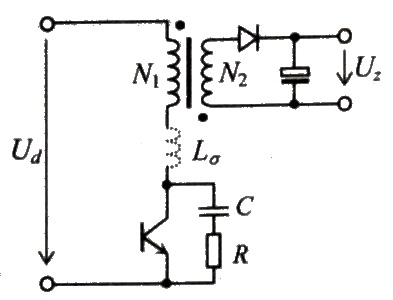
\includegraphics[width=0.4\linewidth]{flyback01.png}}              &
        \subfloat[ ]{\label{ENZ:fig_012}
          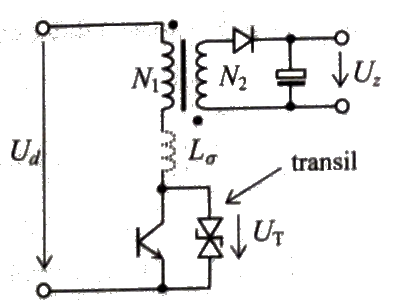
\includegraphics[width=0.4\linewidth]{flyback02.png}}              \\
      \end{tabular}
      \caption{Možnosti potlačení přepětí způsobeného rozptylovou indukčností transformátoru.}
    \end{figure}
    V zapojení podle obr. \ref{ENZ:fig_011} je vhodné vyladit hodnoty prvků \(R\), \(C\) 
    experimentálně 
    pomocí osciloskopu tak, aby byl kmitavý obvod \(R\), \(C\), \(L_\sigma\) tlumen přibližně 
    kriticky. Na odporu \(R\) se v každém případě ztrácí výkon
    \begin{equation}\label{ENZ:eq_032}
      P_R = 2fW_C = 2f\frac{1}{2}C(2U_d)^2 = 4fCU_d^2,
    \end{equation}
    protože během jednoho pracovního cyklu se kondenzátor přes odpor jednou nabije a jednou 
    vybije. Výkon \(P_R\) může dosahovat relativně velkých hodnot. Z energetického pohledu je 
    výhodnější zapojení podle obr. \ref{ENZ:fig_012}, kde transil musí být dimenzován na výkon
    \begin{equation}\label{ENZ:eq_033}
      P_{trans} = fW_\sigma = \frac{1}{2}L_\sigma I_{\mu1_{max}}^2,
    \end{equation}
    protože během jednoho pracovního cyklu zachycuje pouze energii \(W_\sigma\), což bývá méně 
    než \(2CU_d^2\). Další možností je zapojení podle obr \ref{ENZ:fig_013}. Zde probíhá omezení 
    přepětí na tranzistorech \emph{bezeztrátově}. Činnost měniče zůstává úplně stejná jako v 
    základním zapojení.
    \begin{equation}
      \delta_{max} = 1-\frac{U_d}{U_{CE_{max}}}
    \end{equation}
    \begin{figure}[ht!]
      \centering
      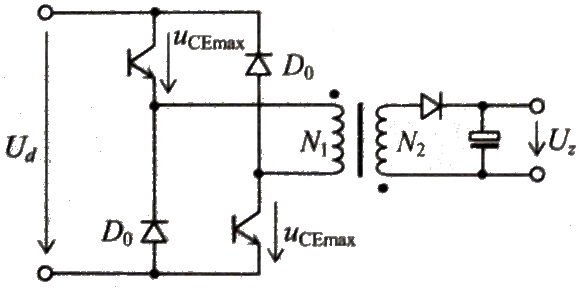
\includegraphics[width=0.7\linewidth]{flyback_2T.png}
      \caption{Přepětí způsobené rozptylovou indukčností transformátoru je potlačeno použitím 
               dvou tranzistorů se záchytnými diodami \(D_0\).}
      \label{ENZ:fig_013}
    \end{figure} 
    Jedná se o dva spínače zapojené do série a spínané současné, jako by se jednalo o spínač 
    jediný. Záchytné diody \(D_0\) slouží pouze k omezení přepětí na tranzistorech, tj. k 
    bezeztrátovému odvedení energie \(W_\sigma\) do ss. meziobvodu. Diody nesmí ovlivňovat 
    činnost měniče. To ovšem znamená, že na jednom tranzistoru musí být ve vypnutém stavu napětí 
    \(U_{CE_{max}}\leqq U_d\), tedy na dvou tranzistorech zapojených v sérii musí být 
    \(2U_{CE_{max}}\leqq 2U_d\). Z rovnice (\ref{ENZ:eq_030}) plyne, že maximální střída musí být 
    omezena na hodnotu
    \begin{align}\label{ENZ:eq_034}
      \delta_{max} &= 1-\frac{U_d}{U_{CE_{max}}} \qquad \rightarrow   \nonumber \\
      \delta_{max} &= 1-\frac{U_d}{2U_{CE_{max}}} = 1 - \frac{U_d}{2U_d} = \frac{1}{2}.
    \end{align}
    Pro případ \(\delta > 0,5\) je zapojení nepoužitelné, protože pak by na každém z tranzistorů 
    muselo být napětí \(U_{CE} > U_d\), což diody \(D_0\) nedovolí.  
